%%
%% $Id$
%%
%% Copyright (c) 2007-2008 Christian Fehler
%% Copyright (c) 2007-2008 Benjamin Mies
%%


\chapter{Minimieren}\label{Minimize}

Wenn wir einen Automaten erstellt haben, können wir mit diesem schon alle
Funktionen, welche dieses Lernwerkzeug bietet, nutzen. Allerdings besteht die
Möglichkeit, dass ein Automat existiert, der die gleiche Sprache erkennt die
unser erstellter Automat erkennt, jedoch mit weniger Zuständen auskommt. Bei
komplexeren Beispielen bemerkt man schnell, dass die Übersichtlichkeit mit
wachsender Anzahl der Zustände immer weiter abnimmt. Daher ist es wünschenswert
immer mit dem minimalen Automaten für eine bestimmte Sprache zu arbeiten. Im
folgenden wollen wir uns jetzt den Algorithmus ansehen, welcher verwendet wird,
um aus einem Automaten einen neuen Automaten mit einer minimalen Anzahl von
Zuständen zu erzeugen.\vspace{10pt}

Wie bereits erwähnt, erhält der Algorithmus als Eingabe einen Automaten, und als
Ausgabe erwarten wir einen Automaten der die gleiche Sprache akzeptiert wie
unser Eingabeautomat, jedoch mit so wenig wie möglich Zuständen
auskommt.\vspace{10pt}

Unser erster Minimierungsschritt besteht darin, die Zustände zu entfernen, die
ausgehend vom Startzustand nicht erreichbar sind. Denn wenn die Zustände nicht
erreicht werden, können sie auch keine Auswirkung auf die Sprache haben, welche
der Automat erkennt. Der dazu verwendete Algorithmus zur Berechnung der
erreichbaren Zustände kann im Abschnitt \ref{ReachableStates} nachgeschlagen
werden.\vspace{10pt}

Im Weiteren versuchen wir äquivalente Zustände in Gruppen, auch
Äquivalenz\-klassen genannt, zusammenzufassen, um diese später zu einem Zustand
zu verschmelzen. Initial wird unsere Menge von Zuständen in zwei Gruppen
unterteilt. Alle akzeptierenden Zustände bilden die erste, alle nicht
akzeptierenden Zustände die zweite Gruppe.\vspace{10pt}

Wir nehmen uns jetzt das Alphabet unseres Eingabeautomaten zur Hilfe, um zu
prüfen, ob alle Zustände einer Gruppe wirklich in einer Äquivalenzklasse
liegen, oder ob wir die Gruppe aufspalten können. Dazu sei gesagt, dass zwei
Zustände in der selben Äquivalenzklasse liegen, wenn sie mit jeweils allen
Symbolen des aktuellen Alphabets in einen Zustand der selben Gruppe
übergehen.\vspace{10pt}

\begin{figure}[h]
\begin{center}
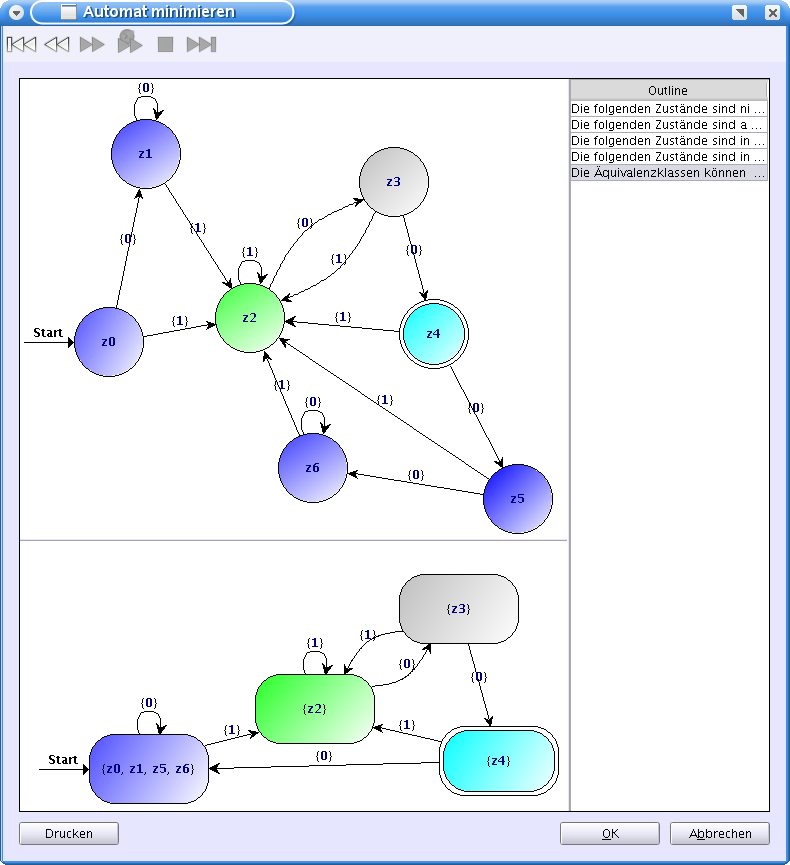
\includegraphics[width=12cm]{../images/minimize.png}
\caption{Automat - Minimieren}
\end{center}
\end{figure}
\vspace{10pt}

Schauen wir uns jetzt mal die Arbeitsweise des Algorithmus im Detail an. Als
erstes müssen wir uns die aktuelle Gruppeneinteilung merken, also wieviele
Gruppen wir haben, und welcher Zustand in welcher Gruppe liegt. Wir betrachten
die erste unserer Gruppen. Wenn diese nur einen Zustand enthält kann sie nicht
weiter verfeinert werden, und muss daher auch nicht mehr betrachtet werden.
\vspace{10pt}

Wenn die Gruppe mehr als einen Zustand beinhaltet, nehmen wir uns das aktuelle
Alphabet des Automaten zur Hilfe. Wir prüfen jetzt für jedes Symbol des Alphabets
einzeln, ob alle Zustände der Gruppe mit diesem Symbol in Zustände der selben
Gruppe übergehen. Wenn das der Fall ist, kann auch diese Gruppe nicht weiter
unterteilt werden. Falls wir aber doch auf Zustände treffen, welche in eine
andere Gruppe übergehen, werden diese Zustände aus der aktuellen Gruppe entfernt
und bilden eine neue Gruppe. \vspace{10pt}

Nachdem wir diese Prozedur für diese Gruppe
abgeschlossen haben, wiederholen wir sie für alle Gruppen die wir noch nicht
betrachtet haben. Nach Betrachtung aller Gruppen vergleichen wir die aktuelle
Gruppeneinteilung mit der, die wir uns gemerkt haben. Wenn diese übereinstimmt,
ist unser Algorithmus am Ende, und die Gruppen können nicht weiter verfeinert
werden. Stimmt die Gruppeneinteilung nicht überein, müssen wir wieder jede
Gruppe einzeln betrachten, und versuchen diese in kleinere Gruppen zu
zerlegen.\vspace{10pt}

Nach Beendigung des Algorithmus repräsentiert jede Gruppe einen Zustand
in unserem neuen Automaten. Jetzt muss noch pro Symbol des Alphabets der
Übergang in den entsprechenden neuen Zustand angelegt werden. Mit diesem
letzten Schritt ist die Konstruktion des minimalen Automaten
abgeschlossen.\vspace{10pt}

In unserem Lernwerkzeug wird dem Benutzer in einer sogenannten Outline genau
mitgeteilt, was in den bisherigen Schritten des Algorithmus passiert ist.
Desweiteren ermöglichen wir dem Benutzer eine schrittweise Navigation und das
Navigieren in Vor- und Rückrichtung. Diese beiden Features sollen es ermöglichen
den Minimierungsalgorithmus besser nachvollziehen und verstehen zu
können.\vspace{10pt}
